\documentclass[10pt,a4paper, landscape]{report}

\usepackage[utf8]{inputenc}
\usepackage{color}
\usepackage{colortbl}
\usepackage{xcolor}
\usepackage{graphicx}
\usepackage[normalem]{ulem}
\definecolor{gris}{rgb}{0.75,0.75,0.75}
\usepackage[top=1cm, bottom=2cm, left=0.5cm, right=0.5cm]{geometry}

\author{Nicolas REYNAUD}
\title{Manuel d'utilisation}
\date{\vfill 09 Mars 2015}

\parindent=0pt

\begin{document}

\maketitle
\newpage


\renewcommand{\contentsname}{Sommaire}
\tableofcontents
\newpage

\center
\section{\uuline{L'accueil}}

Avant toute chose, nous devons nous rendre sur la page d'accueil. Sur celle ci est demandé une autorisation de Géo-localisation.\\
L'application étant entièrement basé sur ceci nous nous devons de la partager.\\
{%
\setlength{\fboxsep}{0pt}%
\setlength{\fboxrule}{2pt}%
\fbox{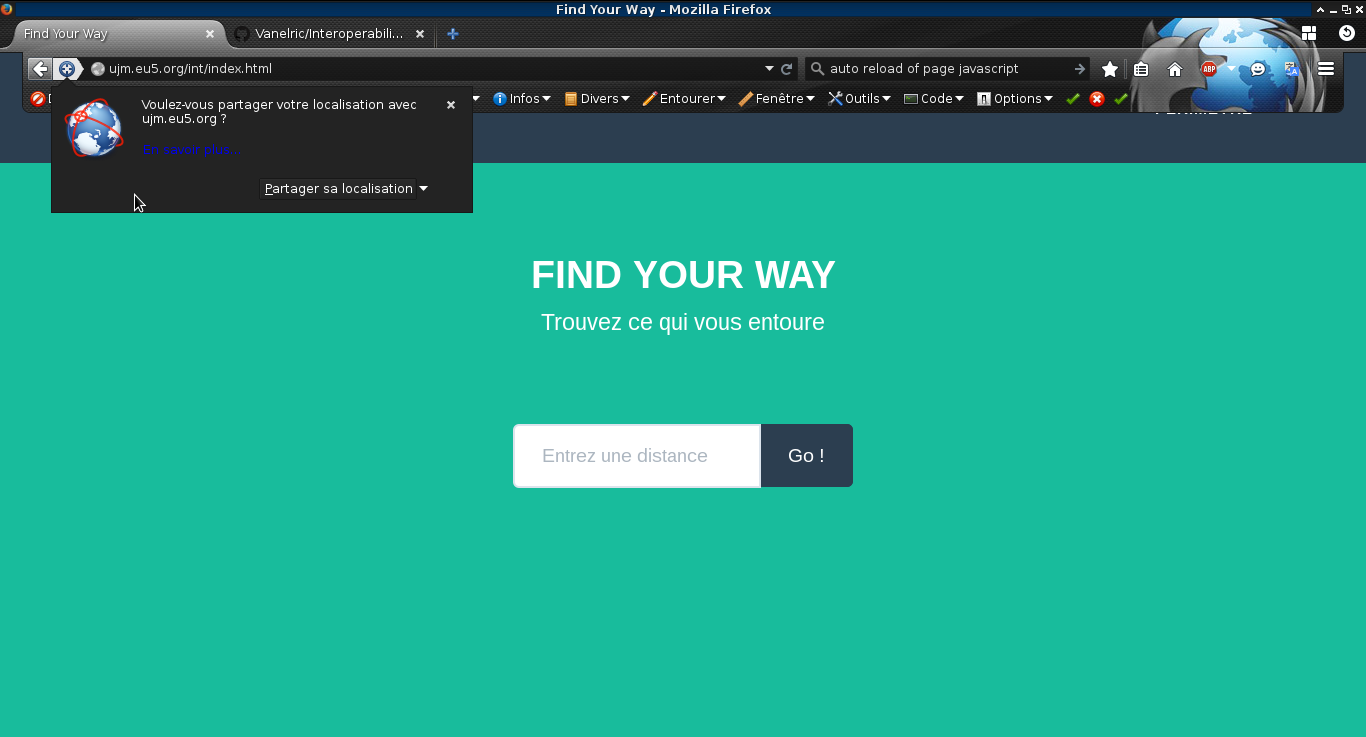
\includegraphics[scale=0.5]{images/accueil_demande.png} %
}%

\newpage
Une fois celle-ci autorisé nous remplissons le champs pour le rayon dans lequel nous cherchons les différents lieux. \\
Puis validons le formulaire en cliquant simplement sur "Go !" \\
{%
\setlength{\fboxsep}{0pt}%
\setlength{\fboxrule}{2pt}%
\fbox{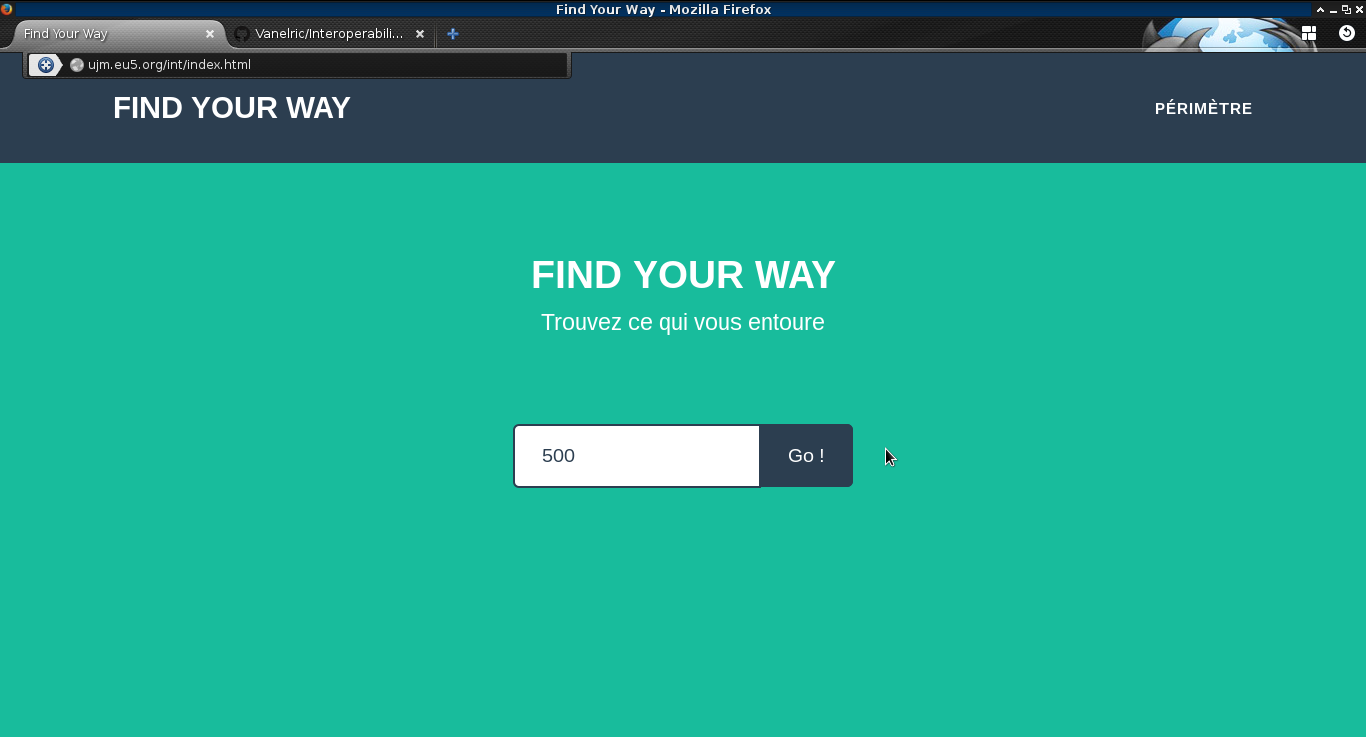
\includegraphics[scale=0.5]{images/accueil_rempli.png} %
}%

\newpage
\section{\uuline{Le choix}}

Une fois le click effectué, nous somme redirigé sur la page qui nous montre la carte. \\
Nous avons donc une liste non-exhaustive des lieux qui nous entour ( google map limitant a 20 curseurs sur la carte ). \\
{%
\setlength{\fboxsep}{0pt}%
\setlength{\fboxrule}{2pt}%
\fbox{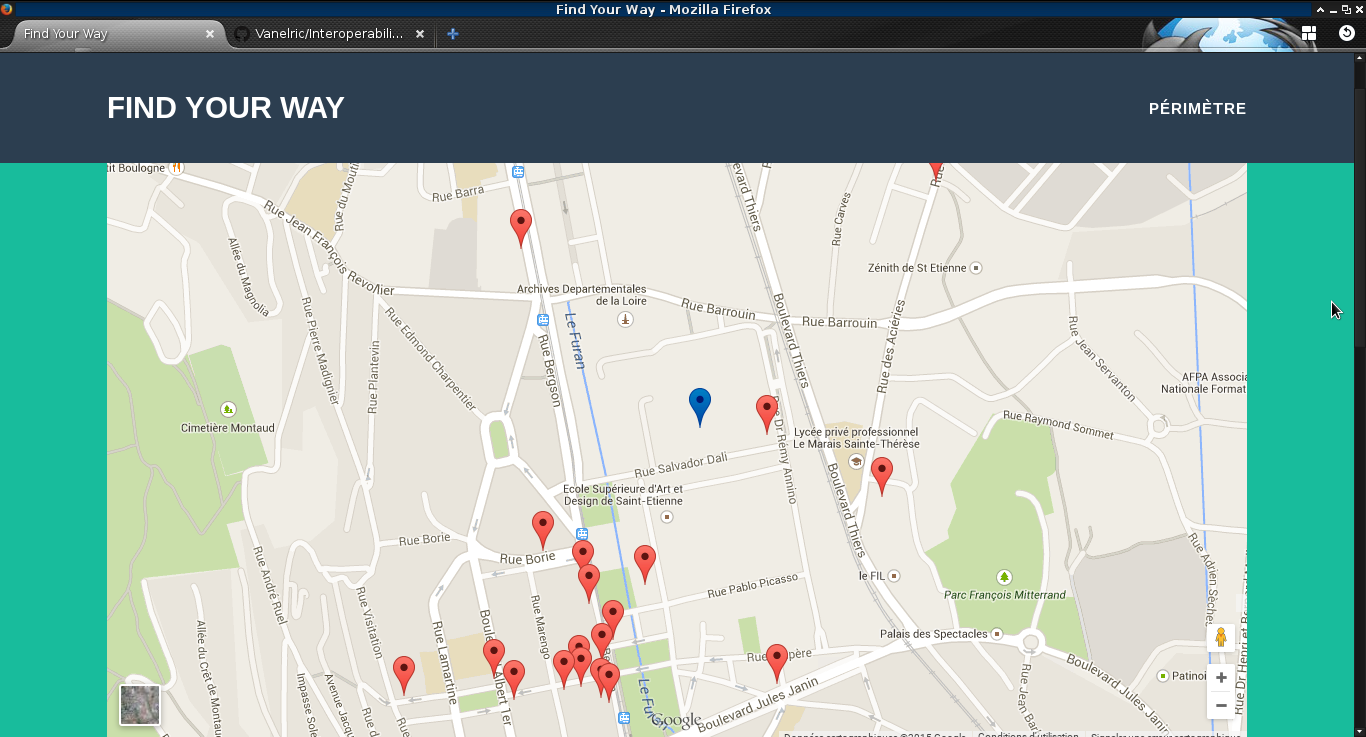
\includegraphics[scale=0.5]{images/map.png}%
}%

\newpage
En "scrollant" alors sur la page nous pouvons accéder aux choix. \\
Par exemple regardons les bars autour de la faculté des sciences, sur le campus carnot. \\
{%
\setlength{\fboxsep}{0pt}%
\setlength{\fboxrule}{2pt}%
\fbox{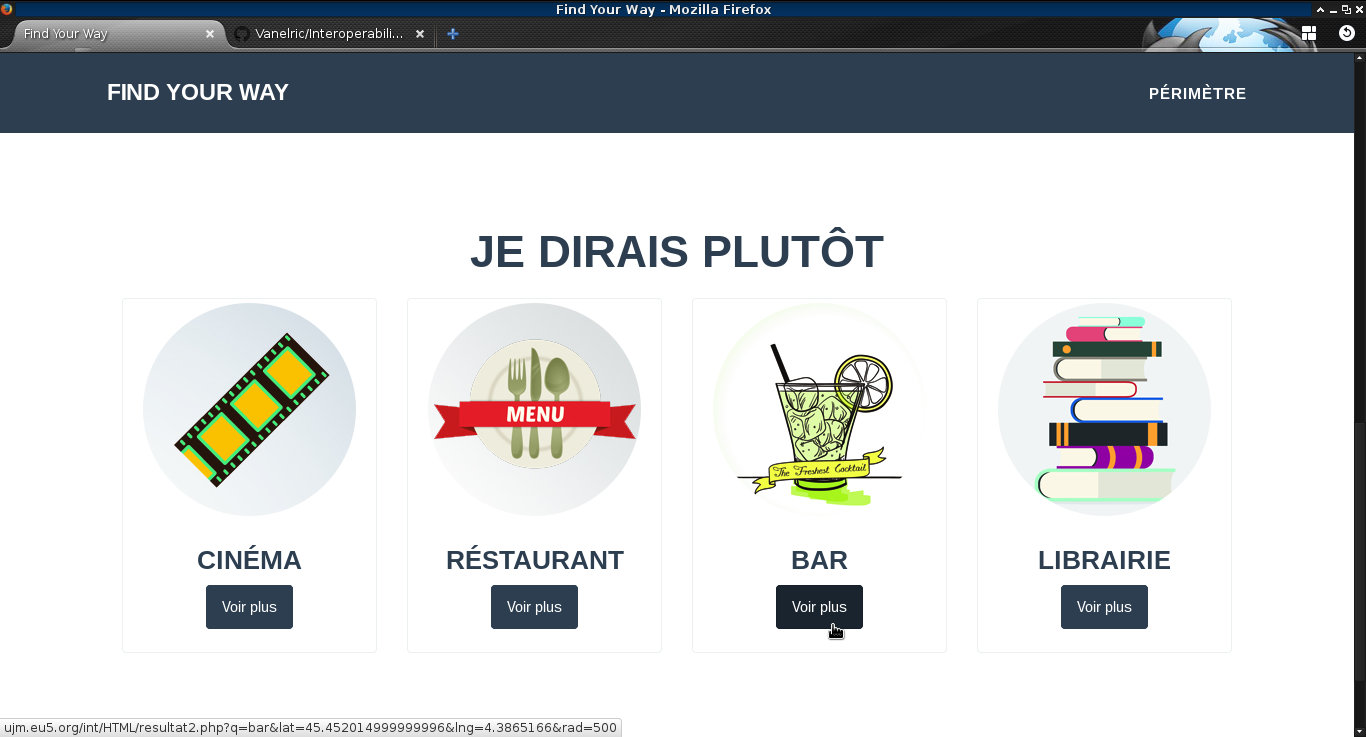
\includegraphics[scale=0.5]{images/choix.png} %
}%

\newpage
\section{\uuline{Vote et affichage}}

Ici nous voici enfin sur la liste des commerces proche de nous, les distances ainsi que l'adresse sont affiché. \\
Nous pouvons également cliquer sur le nom du commerce pour avoir plus d'information sur celui ci. \\
Par exemple dans les cinémas, la liste des films ainsi que les horaires de diffusions de ceci seront indiqué. \\
Dans la partie "Librairie" une liste des nouveaux films sera affiché. \\
Enfin dans la partie "Bar" une liste des cocktails de saisons sera affiché avec leurs ingrédients. \\
{%
\setlength{\fboxsep}{0pt}%
\setlength{\fboxrule}{2pt}%
\fbox{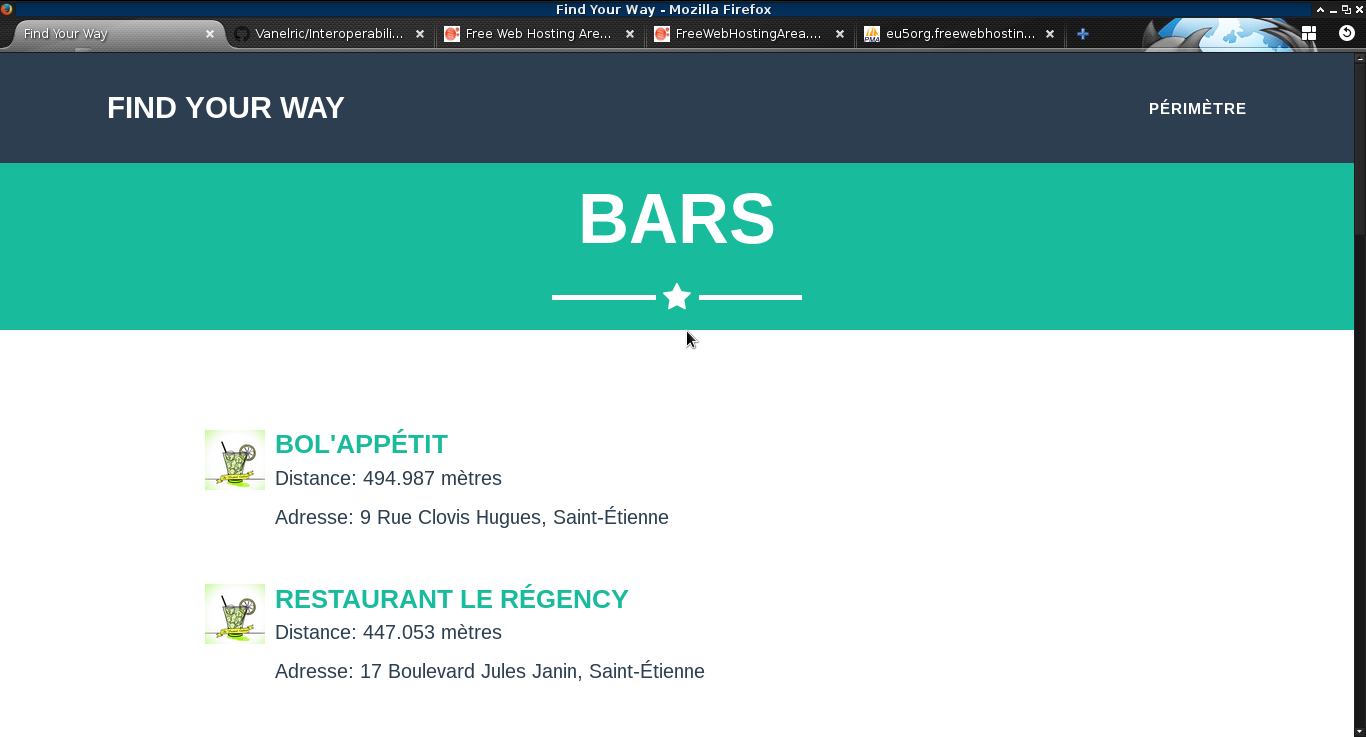
\includegraphics[scale=0.5]{images/bar_liste.png} %
}%

\newpage
Nous voici, après avoir cliqué sur le titre du bar "Bol' Appétit" une liste de cocktail mais également la possibilité de voter pour se bar. \\
Afin d'indiquer aux autres si celui ci est bien ou pas. \\
{%
\setlength{\fboxsep}{0pt}%
\setlength{\fboxrule}{2pt}%
\fbox{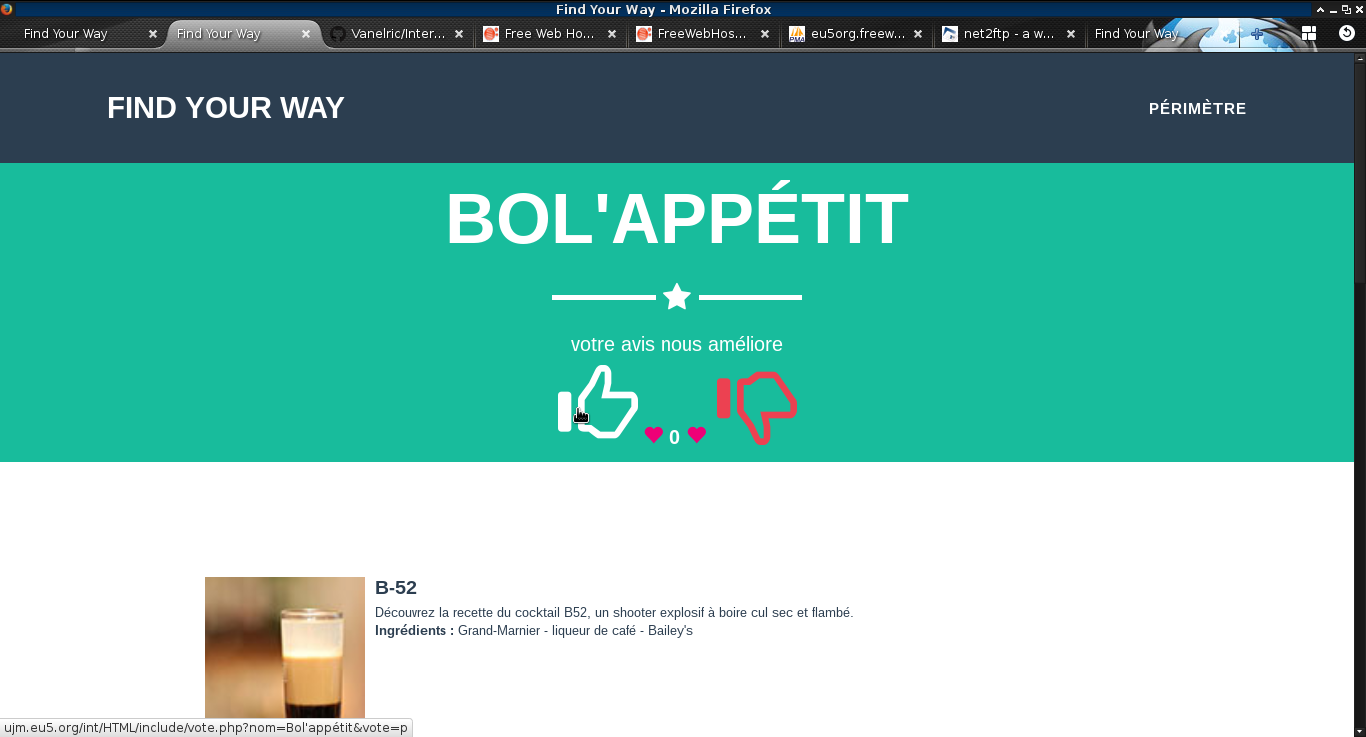
\includegraphics[scale=0.5]{images/cocktail.png} %
}%

\newpage
Une fois le vote effectué, les boutons pour le vote sont caché, ainsi seul le total de vote reste affiché.
Un vote plus augmentera de 1 le nombre de "j'aime" \\
Un vote négative appliquera -1 sur le total de personne ayant aimé ce bar. \\

Un mauvais bar aura dès lors une note négatif. \\
{%
\setlength{\fboxsep}{0pt}%
\setlength{\fboxrule}{2pt}%
\fbox{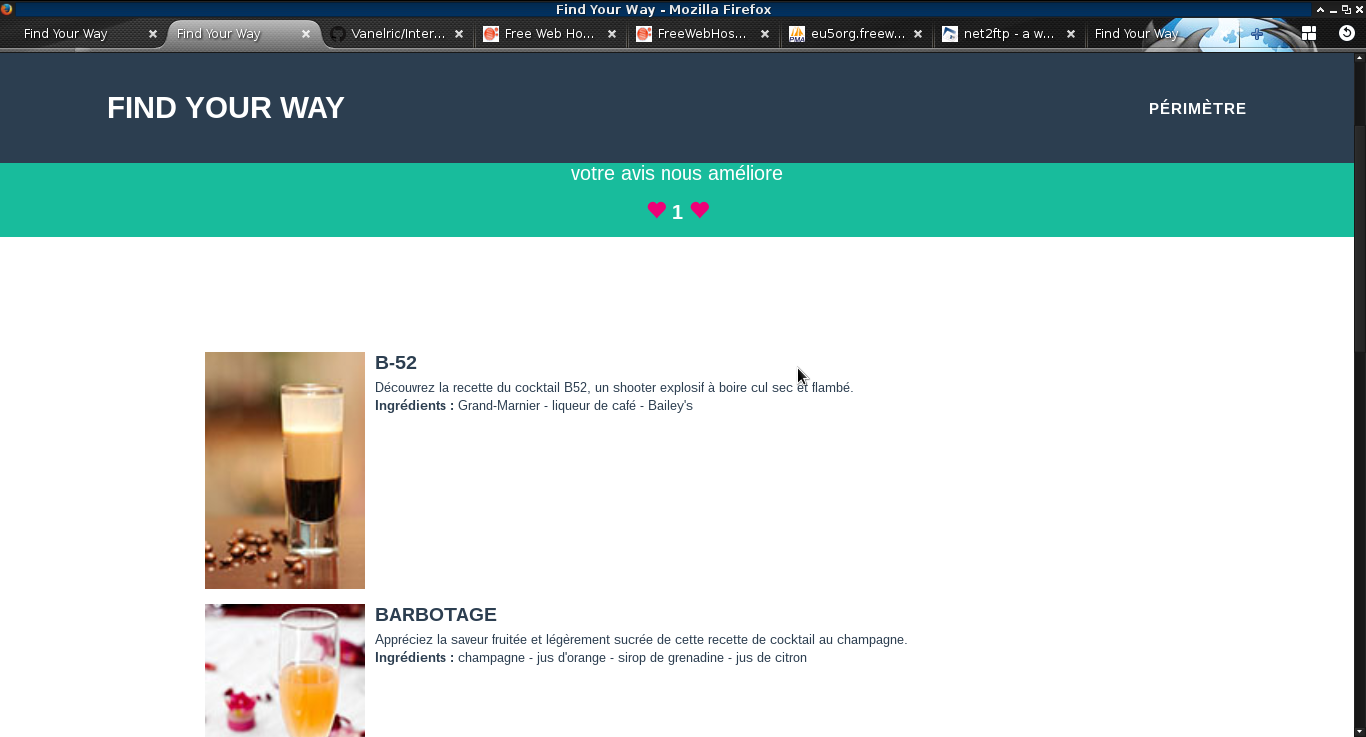
\includegraphics[scale=0.5]{images/vote.png} %
}%

\newpage
\section{\uuline{Ajout de lieu}}

Supposons maintenant que notre lieu favoris n'est pas présent dans la liste des bars, ou la liste des librairies etc.. \\
Nous pouvons l'ajouter en cliquant simplement sur le bouton "Ajouter un lieu" un formulaire apparait alors. \\

Nous allons alors ajouté un bar ici nous le nommerons "Carnot Bar" présent a l'adresse de la faculté. \\
Cliquons ensuite sur "Ajouter le lieu".
{%
\setlength{\fboxsep}{0pt}%
\setlength{\fboxrule}{2pt}%
\fbox{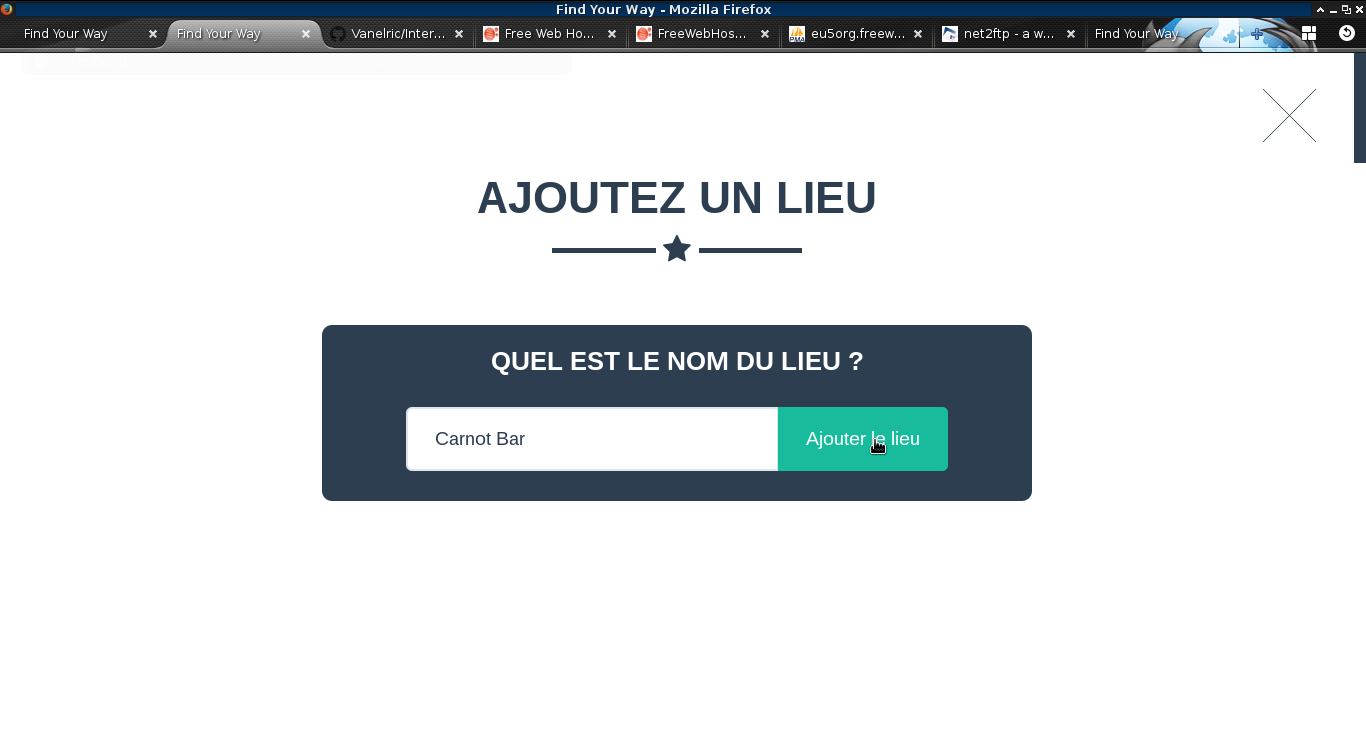
\includegraphics[scale=0.5]{images/ajout_lieu.png} %
}%

\newpage
Un message apparait alors pour nous indiquer que le lieu as bien été ajouté. \\
Dans le cas ou le lieu existe déjà un message nous indique que "Le lieu existe déjà". \\
{%
\setlength{\fboxsep}{0pt}%
\setlength{\fboxrule}{2pt}%
\fbox{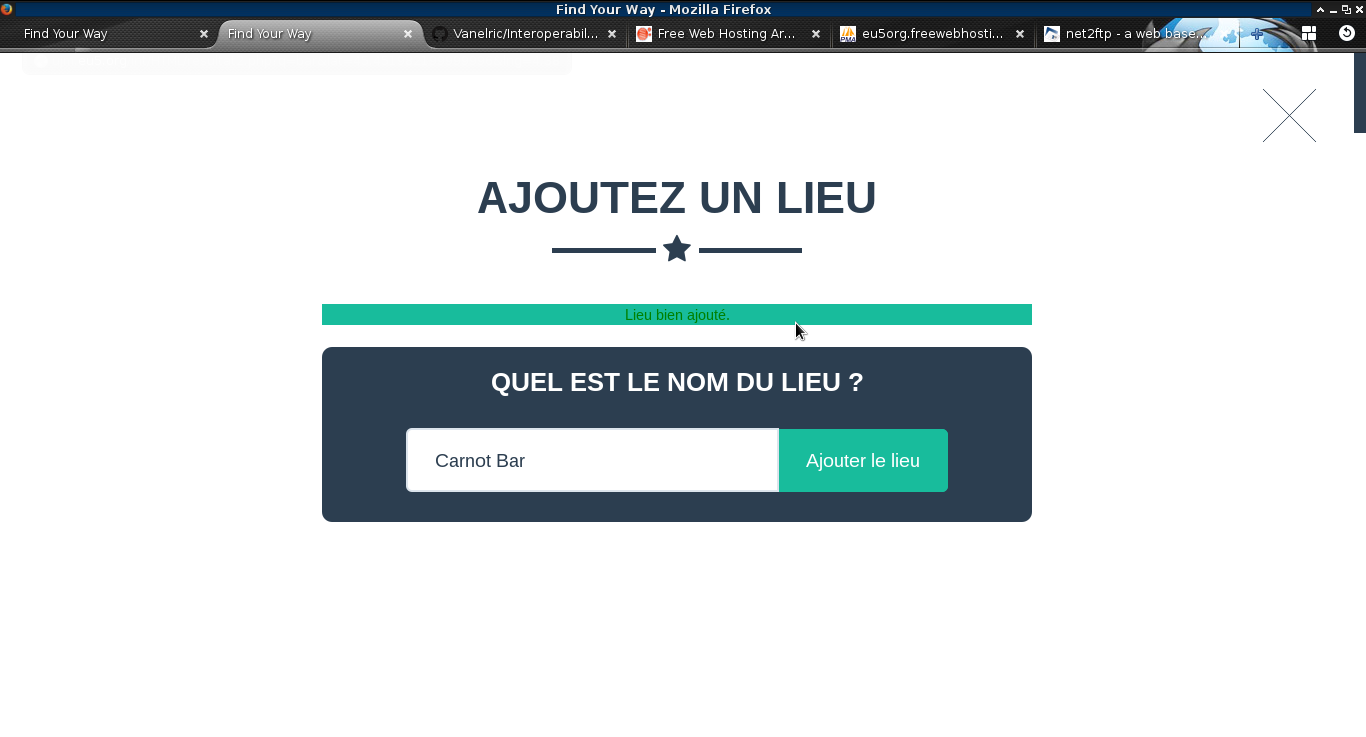
\includegraphics[scale=0.5]{images/good_ajout.png} %
}%

\newpage
Puis après 5 secondes, la page se recharge automatiquement pour nous afficher la nouvelle liste avec le lieu ajouté. \\
{%
\setlength{\fboxsep}{0pt}%
\setlength{\fboxrule}{2pt}%
\fbox{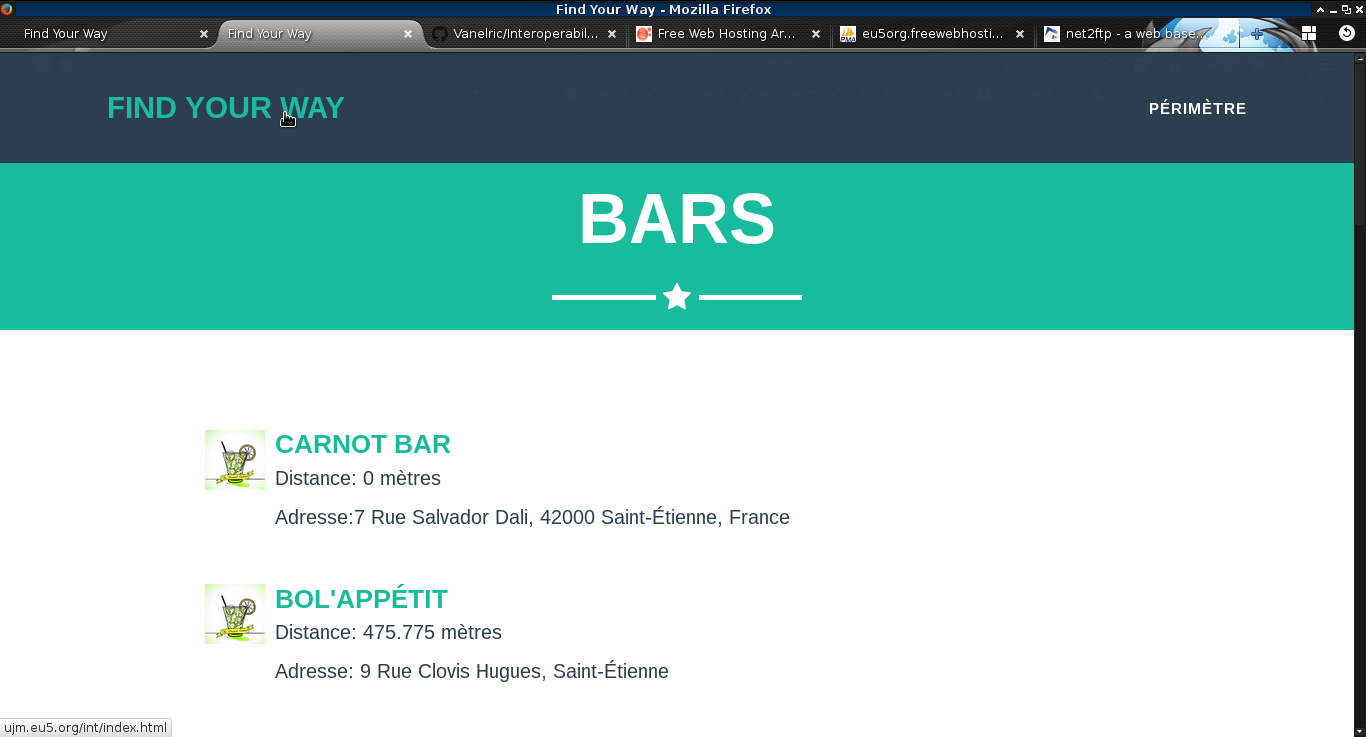
\includegraphics[scale=0.5]{images/carnot_ajouter.png} %
}%

\end{document}